\documentclass[onecolumn, draftclsnofoot,10pt, compsoc]{IEEEtran}

\usepackage{graphicx}
\usepackage{url}
\usepackage{setspace}
\usepackage{pgfgantt}
\usepackage{splitbib}
\begin{category}[A]{Compliance}
  \SBentries{projectDesc,devtargets,opensoundcontrol} %requirements
\end{category}
\begin{category}[B]{Guidance}
  \SBentries{} %extra
\end{category}

\usepackage{geometry}
\geometry{textheight=9.5in, textwidth=7in}



% 1. Fill in these details
\def \CapstoneTeamName{		        The Slide Sentinel}
\def \CapstoneTeamNumber{		    29}
\def \GroupMemberOne{			    James Stallkamp}
\def \GroupMemberTwo{			    Lucas Campos-Davis}
\def \GroupMemberThree{			    Kevin Koos}
\def \CapstoneProjectName{		    Slide Sentinel}
\def \CapstoneSponsorCompany{	    Oregon State University}
\def \CapstoneSponsorPerson{		Dr Chet Udell}

% 2. Uncomment the appropriate line below so that the document type works
\def \DocType{	%Problem Statement
				Requirements Document
				%Technology Review
				%Design Document
				%Progress Report
				}
			
\newcommand{\NameSigPair}[1]{\par
\makebox[2.75in][r]{#1} \hfil 	\makebox[3.25in]{\makebox[2.25in]{\hrulefill} \hfill		\makebox[.75in]{\hrulefill}}
\par\vspace{-12pt} \textit{\tiny\noindent
\makebox[2.75in]{} \hfil		\makebox[3.25in]{\makebox[2.25in][r]{Signature} \hfill	\makebox[.75in][r]{Date}}}}
% 3. If the document is not to be signed, uncomment the RENEWcommand below
\renewcommand{\NameSigPair}[1]{#1}

\bibliographystyle{IEEEtran}


%%%%%%%%%%%%%%%%%%%%%%%%%%%%%%%%%%%%%%%
\begin{document}



% forces all bib entries to show
\nocite{*}

\begin{titlepage}
    \pagenumbering{gobble}
    \begin{singlespace}
        \hfill 
        % 4. If you have a logo, use this includegraphics command to put it on the coversheet.
        %\includegraphics[height=4cm]{CompanyLogo}   
        \par\vspace{.2in}
        \centering
        \scshape{
            \huge CS Capstone \DocType \par
            {\large\today}\par
            \vspace{.5in}
            \textbf{\Huge\CapstoneProjectName}\par
            \vfill
            {\large Prepared for}\par
            \Huge \CapstoneSponsorCompany\par
            \vspace{5pt}
            {\Large\NameSigPair{\CapstoneSponsorPerson}\par}
            {\large Prepared by }\par
            Group\CapstoneTeamNumber\par
            % 5. comment out the line below this one if you do not wish to name your team
            \CapstoneTeamName\par 
            \vspace{5pt}
            {\Large
                \NameSigPair{\GroupMemberOne}\par
                \NameSigPair{\GroupMemberTwo}\par
                \NameSigPair{\GroupMemberThree}\par
            }
            \vspace{20pt}
        }
        \begin{abstract}
        	This document outlines the requirements for the Slide Sentinel 2018-19 senior capstone project. This document includes both the requirements for the Slide Sentinel and ONE hub projects this team will be working on. Outlined below is the requirements of the projects software for both hubs and the online client.
        \end{abstract}     
    \end{singlespace}
\end{titlepage}



\newpage
\pagenumbering{arabic}
\tableofcontents
\clearpage



\section{Introduction}
Environmental sensing data is used extensively by both scientists and engineers for a variety of uses such as research, risk analysis, and many others. It is common for such data to come from remote locations where there isn't constant human presence, so a way of collecting this data remotely would be extremely convenient and practical. The ONE hub from the OSU Open Sensing lab seeks to provide such a way to not only remotely communicate with a sensing project, but also to interface with other sensors wirelessly for data collection.
\\* \\*
Landslides are costly for land management to deal with due to their expensive clean up costs and the remote nature of most landslides. Monitoring the mass movement of geography can be used to accurately predict the likelihood of future landslides and track historical movements. Slide Sentinel is a project which will provide such a way to collect this data and remotely send it to the cloud for storage and future visualization. This project is a derivative project of the ONE hub and LOOM sensors in principle, but due to constraints, these projects are actually vastly different from one another.


\subsection{Purpose}
The Slide Sentinel system seeks to provide a method for land management owners to accurately monitor and track information about mass movement in remote mountainous locations. The system will track the positions of sensor nodes and communicate any changes in position to a larger database or spreadsheet. This information can then be accessed by the client for further analysis and shown in a Google maps visual of the positional changes.
\\* \\*
The goal of the LOOM project at the OSU Open Sensing lab is to provide a framework for scientists and engineers to deploy sensing projects and collect information. The Project LOOM enables users to easily prototype and create new sensing projects through its plug-and-play software and modularity of the boards. One of the primary uses of sensing projects is to gather environmental data from a remote location. The ONE hub will be added to this ecosystem of sensors to enable users to remotely collect data from a project in a remote area as well as communicate with other sensors over WiFi, LoRa, or nRF. The hub will also be capable of sending the data over WiFi, 4G LTE, or satellite communication. 

\subsection{Scope}
%explain the system including identifying information on names, function, benefits,
Starting from the bottom, the Slide Sentinel sensors are microcrontrollers with wireless radio capabilities along with an accelerometer module.
The central hub consists of some microtroller which is outfitted to collect radio communication from the sensor array and send data over SatCom or 4G LTE periodically to a larger database. 4G LTE will be used as a less expensive option to satellite communication when networks are available. Data will be collected in a Google sheet for detailed viewing. This data will then be used to construct a Google maps visualization to track the paths of sensors over time.
\\* \\*
The ONE hub will consist of a wirelessly enabled microcontroller along with an assortment of antennae for various wireless radio capabilities. It will be capable of communicating with other LOOM systems over WiFi, LoRa, and nRF. The hub will be capable of transmitting this information using either 4G LTE, WiFi, or satellite connection to another service which can route the data to other specified repositories.


\subsection{Product Overview}
\subsubsection{Overview}
%full explanation of system
Slide Sentinel is a system of sensors, transmitters, and internet applications that collect, upload, and present data on land slide activity. Slide Sentinel is composed of multiple devices and applications that work together to detect land slides, the main components are the sensor modules, a hub module, and an online application. The sensor module and hub module are physical devices placed in land slide prone areas which will collect positional data on local landslides. The sensors will be provided correctional positioning data from the hub to increase their accuracy. The sensor module will detect changes in its position or orientation and send this data to the central hub. Periodically this data will be sent over a satellite or 4G LTE connection to an online spreadsheet application. The data can then be used by users for analysis and be shown in an online mapping application for easy viewing. The viewing application will provide information such as id, position, and status as well as a way to view the historical positions of the sensors.
\\* \\*
ONE hub is a wireless hub which is designed to be used in the LOOM ecosystem of sensors and software. The hub will be capable of communicating with other machines over WiFi, LoRa, and nRF. This hub will also be capable of connecting to a 4G cellular network, local WiFi, or satellite so users can manage their project or have their collected data sent somewhere else using a cloud notification API.

\subsubsection{Perspective}
%how is our product related to a larger system (does not apply to slide sentinel but is important in one hub), and how does %it interface with it. What are the major elements of the system and how do they all interface with each other
%what are our constraints from the system, user, hardware, software, etc. interfaces

The Slide Sentinel system consists of the three major elements. There are the sensors which collects information, the wireless hub, and a visualization web page. The sensors communicate with the wireless hub over a radio connection and the hub transmits data elsewhere over a satellite connection or cellular network.
\\* \\*
The ONE hub will integrate with the LOOM library in order to provide the networking capabilities of the hub to the larger ecosystem of LOOM sensor modules. The hub will comply with all specifications and guidelines of the LOOM library including the Open Sound Control(OSC) specification. The hub in total consists of a wirelessly enabled microcontroller and any number of radio modules and antennae for communicating with LOOM sensors over WiFi, LoRa, or nRF. Outgoing communication can be WiFi, 4G LTE, or satellite communication.

\subsubsection{Functions}
%what functions does our product provide to end users
The Slide Sentinel system will allow users to track and visualize the movement of sensors deployed in strategic locations to collect landslide information. Users will be able to access this information in a plain text format through an online spreadsheet application which will show information about individual sensors such as id, longitude, latitude, orientation, status, and a time stamp of the last data collection. A mapping application will be used to provide a way to visualize this information geometrically on a map for easy viewing.
\\* \\*
%end-user functions of ONE hub
The ONE hub will allow users to connect an array of LOOM sensor modules to the ONE hub for combined data transmission. The ONE hub will allow users to connect LOOM sensor modules over WiFi, LoRa, and nRF. The ONE hub will then be able to transmit data collected from these sensor modules to a remote location over a 4G cellular network, WiFi, or satellite connection.


\subsubsection{User Characteristics}
%specify characteristics of the user interface and how it might be optimized for the kind of end user who uses the product
%important for slide sentinel, difficult to say for the one hub but i think the configuration file and how it looks in the
%loom software might fit
The primary user of Slide Sentinel is researchers working on monitoring or preventing landslides. This user will most likely have some technical background but not necessarily related to computers. Given the background of the users the online client can present scientific data in a plane manner, however the website should still be simple to use because the user might not have a background in computers. This user mostly cares about being able to see a visualization of how land has shifted and possibly access to the raw data itself. This means the primary focus of the user interface will be the visualization functionality.
\\* \\*
Users of ONE hub are expected to be those with at least a bit of IT expertise in order to use the LOOM software and correctly configure both the software and the ONE hub itself.


\subsubsection{Limitations}
%most of these are the same between both hubs
\begin{itemize}
    \item Hardware \\ %microcontroller choice, battery, antennae
        The hardware configurations for both hubs need to stay under and on budget. This includes choice of microcontroller, communication module, battery, antenna, and enclosure.
    \item Interface \\ %wireless limitations(need LOS of sky for satcom), satcom server to google stuff, nb-iot to pushingbox
        The Slide Sentinel hub needs enough open space to connect to a satellite communication or 4G LTE network.
    \item Quality \\ %reliability and battery life, more information on google drive
        The battery chosen needs to be able to power the hardware configuration for at least three months. The hub needs to upload data on a consistent schedule.
\end{itemize}


\section{References}
\bibliography{bibliography.bib}

\section{Specific Requirements}
%only some of these sections will need to be filled out, likely only 

\subsection{External Interfaces} %requirements on handling interrupts?
\subsubsection{Hardware Interface}
Both hubs will allow for users to manually retrieve data if the long range wireless connection is not functional. Data will be stored on a memory card and can be accessed through a universal serial connection.  

\subsubsection{User Interface}
The online client will provide the only user interface. The online client is a web page that must be portable to most modern web browsers. The online client will display collected data over a projection of the related area where the sensors are located. This visualization will show users how the sensors have shifted in position or orientation over time. The online client will also make raw data available to the user for inspection or retrieval.

\subsection{Logical Database}
The system will frequently push data to an online spread sheet application. This data will be kinematic data from the sensor components, this data will be formatted to fit into a spread sheet.

\subsection{Performance Requirements} %battery life, efficiency, etc
The hub and sensor components must be optimized to perform well in remote locations. In order to operate in remote locations for extended periods both the hub and the sensor components need to be very power efficient. The hub and sensor components are both used to transmit data and must balance power efficiency and performance in order to be able to upload all the necessary data.

\subsection{Enclosure Design Constraints} %something on the requirements for the enclosure
The Slide Sentinel hub will include an enclosure in the final product which can withstand outside weather conditions. The enclosure should provide protection against dust particles, water, and small impacts due to blown twigs and branches. The enclosure will be 3D-printed to reduce the overall cost of the project and allow for replacements to be readily constructed. This is equivalent to around an IP54/55 rating depending on the water resistance of the enclosure.

\subsection{Supporting Information} %documentation information for use of product, important for both
Documentation on the usage of both hubs will be provided so that any user may understand the specifications of the product and the necessary technologies it supports. Information on the usage of the ONE hub in the LOOM library will also be provided so users can easily use it in LOOM projects.
\begin{figure}[h]
    \centering
    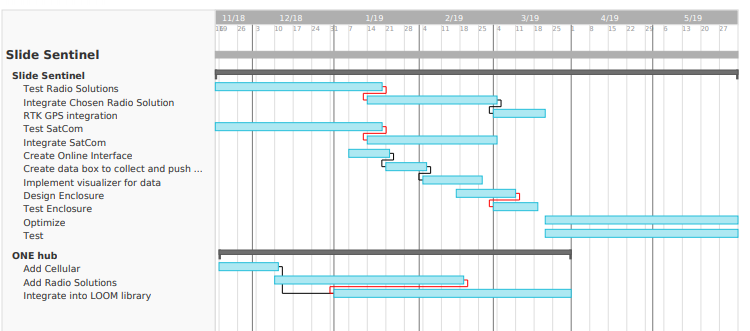
\includegraphics[width=6.5in]{gantt.PNG}
    \caption{Gantt Chart}
    \label{fig:Gantt_Chart}
\end{figure}
\end{document}